\documentclass{standalone}
\usepackage{tikz}

\begin{document}
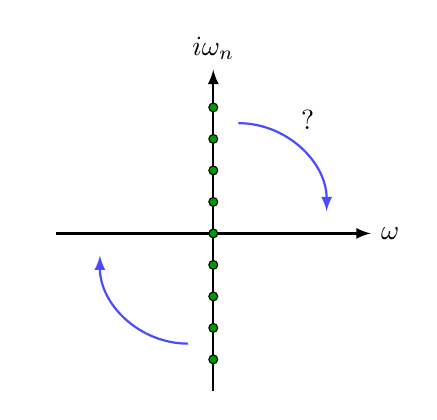
\begin{tikzpicture}[scale=0.8]
  % Draw axes
  \draw[-latex,thick] (-2.5,0) -- (2.5,0) node[right] {$\omega$};
  \draw[-latex,thick] (0,-2.5) -- (0,2.6) node[above] {$i\omega_n$};
  
  % Small black circles
  \draw[fill=green!60!black] (0,0) circle (2pt);
  \draw[fill=green!60!black] (0,0.5) circle (2pt);
  \draw[fill=green!60!black] (0,-0.5) circle (2pt);
  \draw[fill=green!60!black] (0,1) circle (2pt);
  \draw[fill=green!60!black] (0,-1) circle (2pt);
  \draw[fill=green!60!black] (0,1.5) circle (2pt);
  \draw[fill=green!60!black] (0,-1.5) circle (2pt);
  \draw[fill=green!60!black] (0,2) circle (2pt);
  \draw[fill=green!60!black] (0,-2) circle (2pt);
  
  % Circle with arrow
  \draw[-latex,thick,blue!70] (0.4,1.75) arc (90:0:1.4);
  \draw[-latex,thick,blue!70] (-0.4,-1.75) arc (270:180:1.4);
  
  \node at (1.5, 1.8) {?};
  \node at (-2.8, 1.8) {};
  
\end{tikzpicture}
\end{document}